\documentclass[]{article}
\usepackage{fullpage}
\usepackage{graphicx}
\usepackage{mhchem}

\title{Chemistry Notes}
\author{Day Two}
\date{Summer 2011}

\begin{document}

\maketitle

\section{States of matter}
Chemistry studies matter in its various states. The three states we will consider are solid, liquid, and gas. Solids have fixed shape and volume; liquids have fixed volume but variable shape; and gases have variable shape and variable volume.

\section{Physical and chemical properties and changes}
Physical properties are properties inherent to a substance, while chemical properties involve a substances ability to form new substances.

\subsection{Examples}
\vspace{5mm}
\begin{tabular}{ | l | l | }
    \hline
    Property & Type \\ \hline
    Boiling point of water & Physical \\ \hline
    Hardness of diamond & Physical \\ \hline
    Fermentation of sugar to form alcohol & Chemical \\ \hline
    Metal wire conducting electricity & Physical \\ \hline
    Metal melting & Physical \\ \hline
    Paper combusting in air & Chemical \\ \hline
\end{tabular}

\section{Elements and compounds}
Elements are a single type of atom. All of the entries on the periodic table (e.g. oxygen, hydrogen, and iron) are elements. Compounds are specific combinations of multiple different elements. \ce{H20}, \ce{C6H12O6}, and \ce{NaCl} are all compounds.

\subsection{Examples}
\vspace{5mm}
\begin{tabular}{ | l | l | }
    \hline
    Example & Type \\ \hline
    Water (\ce{H2O}) & Compound \\ \hline
    Nitrogen (\ce{N}) & Element \\ \hline
    Glucose (\ce{C6H12O6}) & Compound \\ \hline
\end{tabular}

\section{Mixtures}
Mixtures have variable composition, while pure substances are made up of the same substance throughout. Pure substances are always elements or compounds. Homogeneous mixtures (AKA solutions) are the same throughout, while heterogeneous mixtures differ throughout.

\subsection{Examples}
\vspace{5mm}
\begin{tabular}{ | l | l |}
    \hline
    Example & Type \\ \hline
    Gasoline & Homogeneous mixture \\ \hline 
    Copper & Pure substance \\ \hline
    Air & Homogeneous mixture \\ \hline
    Salt water & Homogeneous mixture \\ \hline
    A stream with gravel at the bottom & Heterogeneous mixture \\ \hline
\end{tabular}

\section{Energy and specific heat}
Energy is different than matter. It is not solid, liquid, or gas. Rather, it is the capacity to do work. Energy can be measured in either joules or calories, with:

1 cal = 4.184 J

To find the specific heat of an object, we use the formula:

$Q = s \times m \times \Delta{T}$

\vspace{5mm}
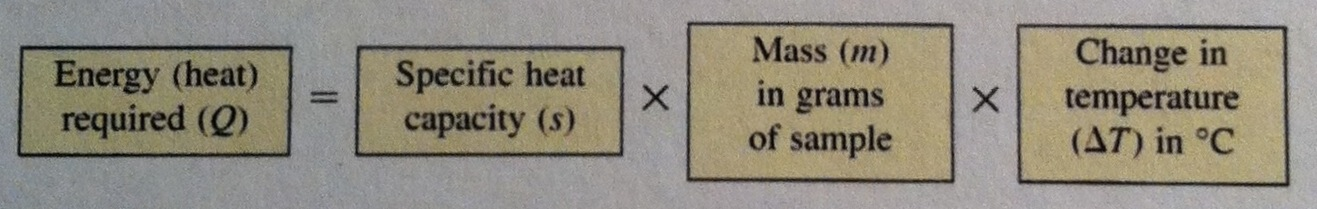
\includegraphics[width=10cm]{specific_heat.jpg}

\section{Atomic theory}
The atom is composed of a tiny nucleus at its center with electrons orbiting around the outside. The nucleus is composed of protons and neutrons.

\vspace{5mm}
\begin{tabular}{ | l | l |}
    \hline
    Particle & Relative charge \\ \hline
    Proton &  +1 \\ \hline 
    Neutron & 0 \\ \hline
    Electron & -1 \\ \hline
\end{tabular}

\section{The periodic table}
% For electron configuration, I attached three figures from page 315 of Zumdahl's Introductory Chemistry: A Foundation, Fourth Edition.
The periodic table contains every element now known to us. It can be used to determine the electron configuration of atoms (see attached figures) and the relative atomic radius of elements. Remember, atomic radius increases from top to bottom, and decreases from left to right.

\vspace{5mm}
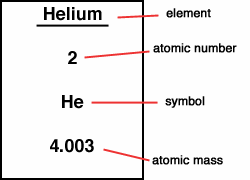
\includegraphics[height=5cm]{helium.png}

\section{Isotopes and allotropes}
Isotopes are different forms of the same element, with different numbers of neutrons. Carbon-12 and carbon-14 are different isotopes of carbon, for example. Allotropes, on the other hand, are different structural forms of an element. Each atom remains unchanged in different allotropes, but the way the atoms are bonded together changes. Graphite and diamond are different allotropes of carbon, for instance.

\section{Ions}
Ions are charged atoms, represented by a plus or a minus sign following the atom's symbol. For instance, a calcium atom that gives up two electrons becomes a \ce{Ca2+} ion, while a chlorine atom that gains an electron becomes a \ce{Cl-} ion.

\section{Acknowledgements}

Some information Zumdahl's \emph{Introductory Chemistry: A Foundation}.

\end{document}
